%laden der Präambel mit Latexbefehlen/-klassen
% !TeX encoding = UTF-8

\documentclass[a0paper,landscape]{baposter}
\usepackage[english]{babel}
\usepackage[utf8]{inputenc}
%\usepackage{arev}
%\usepackage[T1]{fontenc}

\usepackage{marvosym}
\usepackage{pifont}
\usepackage{setspace}

\usepackage{makecell}

%for mathematical symbols
\usepackage{amsmath}
\usepackage{amsxtra}
\usepackage{eurosym}
\usepackage{siunitx}  
\sisetup{locale=DE}
\usepackage[version=4]{mhchem}

%Typography
\usepackage[auto]{microtype}

\usepackage{booktabs}
\usepackage{multirow}
\usepackage{paralist}

\usepackage[
backend=biber,
style=nature,
citestyle=numeric-comp,
sorting=none,
maxbibnames=1,
firstinits=true
]{biblatex}
%\usepackage{natbib}

\bibliography{biblio/refs,biblio/bibtemp}
\setlength\bibitemsep{2.5pt}

%colors
\definecolor{standardfontcolor}{RGB}{0,0,0} 
\definecolor{bordercol}{RGB}{113,113,113}
\definecolor{headercol1}{RGB}{255,255,255}
\definecolor{headercol2}{RGB}{113,113,113}
\definecolor{headerfontcol}{RGB}{0,0,0}
\definecolor{boxcolor}{RGB}{255,255,255}


\begin{document}
	\typeout{Poster rendering started}
	
\background{
	\begin{tikzpicture}[remember picture,overlay]%
	\draw (current page.north west)+(-2em,2em) node[anchor=north west]
	{\includegraphics[height=1.1\textheight]{figures/background}};
	\end{tikzpicture}
}

\color{standardfontcolor}

\begin{poster}{
		grid=false,
		columns=3,
		%colspacing=length
		headerheight=0.125\textheight,
		eyecatcher=false,
        borderColor=bordercol,
		headerColorOne=headercol1,
		headerColorTwo=headercol2,
		headerFontColor=headerfontcol,
		% Only simple background color used, no shading, so boxColorTwo isn't necessary
		boxColorOne=boxcolor,
		headershape=roundedright,
		headerfont=\sffamily\bfseries\Large,
		textborder=rectangle,
		headerborder=open,
		boxshade=plain,
		background=none
%		background=user
	}
	%%% Eye Cacther %%%%%%%%%%%%%%%%%%%%%%%%%%%%%%%%%%%%%%%%%%%%%%%%%%%%%%%%%%%%%%%
	{
		Eye Catcher, empty if option eyecatcher=false - unused
	}
%----------------------------------------------------------------------------------------
%	TITLE AND AUTHOR NAME
%----------------------------------------------------------------------------------------
%
{
	\textsf %Sans Serif
	{\vskip 2.0cm Exploring complex normal faulting systems through \\ physics-based dynamic rupture modeling.}
}
{\sf\vspace{-0.1em}\\
	{\textbf{H.-S. S\'anchez-Reyes$^1$}, O. Scotti$^1$, S. Hok$^1$, A.-A. Gabriel$^2$ and C. Uphoff$^2$}
	\vspace{0.2em}\\
	\normalsize{Bureau d’Évaluation des Risques Sismiques pour la Sûreté des Installations, IRSN, 92260 Fontenay-aux-Roses, France
	\vspace{0.1em}\\
	Department of Earth and Environmental Sciences, Ludwig-Maximilians-Universitat, 80333 Munchen, Germany	 	
	\hskip 1.7cm \textbf{\normalsize \Letter} \textbf{hugo.sanchez-reyes@univ-grenoble-alpes.fr}
	} \\ \\ \\ \\ \\ 
}
% University/lab logo
{ \begin{minipage}{2cm}
  \vskip -0cm \hskip -7.3cm \includegraphics[width=9cm]{../../logos/logo_poster_2022.png}
 \end{minipage}
 }
  %\includegraphics[height=2cm]{../../../../logos/logo_irsn.png}} %
%




\headerbox{{\bf 1.} Introduction}{name=intro,column=0,row=0,span=1}{

\begin{minipage}{0.54\linewidth}
\vskip -1cm
\centering {\bf Norcia-Amatrice-Visso } \vskip 0.4cm 
 \includegraphics[width=1\linewidth]{images/Map_Italy}
\end{minipage}
\begin{minipage}{0.44\linewidth}
 \vskip -0cm {\small {\bf Geological context:}}
 \vskip 0.3cm
 {\small
 \begin{spacing}{1.0}
 
 The Apennine seismic belt in Ita-\\
 ly is an extensional province cha-\\
 racterized by multi-fault normal-\\
 faulting seismic activity. Earth-\\
 quakes and/or seismic sequences \\
 ocurring across multi-fault seg-\\
 ments during a single event (e.g. \\
 1980 Ms 6.9 Irpinia Bernanrd \&\\
 Zollo (1989)) or sequences span-\\
 ning a period of days (e.g. 2009 \\
 Mw 6.1 L’Aquila Valoroso et al \\ 
 (2013)) to months (e.g. 2016 A-\\
 matrice-Visso-Norcia Improta et\\
 al. (2019)), are controlled by the\\
 physical complexities of the acti-\\
 ve normal fault system. \\
 
 Understanding rupture propaga- \\
 tion across step overs, breaking\\
 multiple fault segments during a\\
 single earthquake, is crucial to\\
 enhance the current seismic ha-\\
 zard assessment Bai and Ampue-\\
 ro (2017). \\ \nocite{Bai_2017_ESD} \\
 \end{spacing} 
 }
\end{minipage}
\vskip -0.8cm
   \begin{tikzpicture}[%
    auto,
    block/.style={
      rectangle,
      draw=black,
      thick,
      fill=red!100,
      text width=\textwidth,
      align=justify,
      rounded corners,
      minimum height=3em
    },
    block1/.style={
      rectangle,
      draw=black,
      thick,
      fill=red!20,
      text width=\textwidth,
      align=center,
      rounded corners,
      minimum height=2em
    },
    line/.style={
      draw,thick,
      -latex',
      shorten >=2pt
    },
    cloud/.style={
      draw=red,
      thick,
      ellipse,
      fill=red!20,
      minimum height=1em
    }
  ]
    \draw (2.5,-2) node[block] (C) {\bf \color{white} \footnotesize Goal: Explore dynamic rupture parameters to better understand the physical condition promoting rupture jumps in normal faulting systems};
  \end{tikzpicture}


}



\headerbox{{\bf 2.} Geometry-Settings}{name=geo,column=0,row=1,span=1,below=intro}{

\hskip -0.3cm 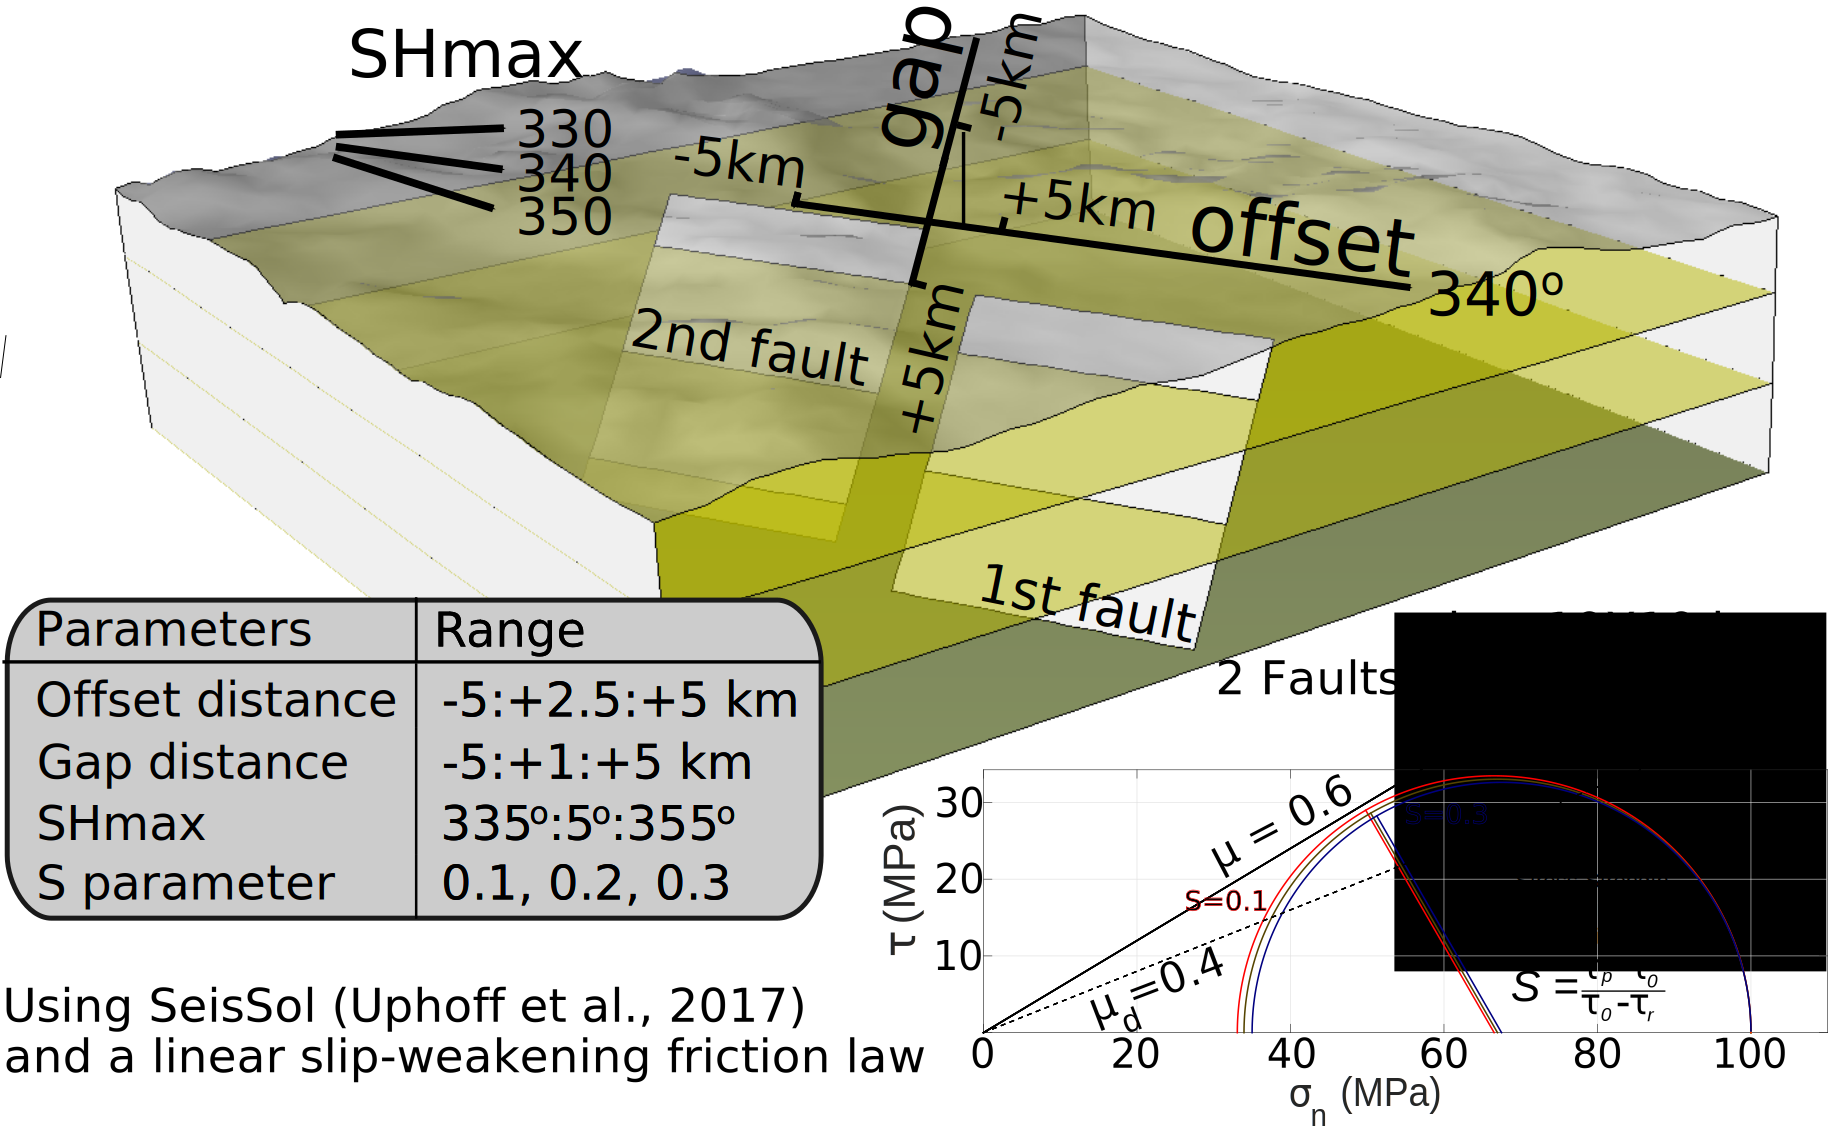
\includegraphics[width=1\linewidth]{images/model.pdf}
\vskip 0.3cm
\begin{center}
 \includegraphics[width=0.75\linewidth]{images/MC_circle_new.pdf} 
\end{center}



}


\headerbox{{\bf 3.} Simulation-Results}{name=summary,column=1,row=0,span=2}{

\begin{minipage}{0.4\linewidth}
\vskip 0.1cm 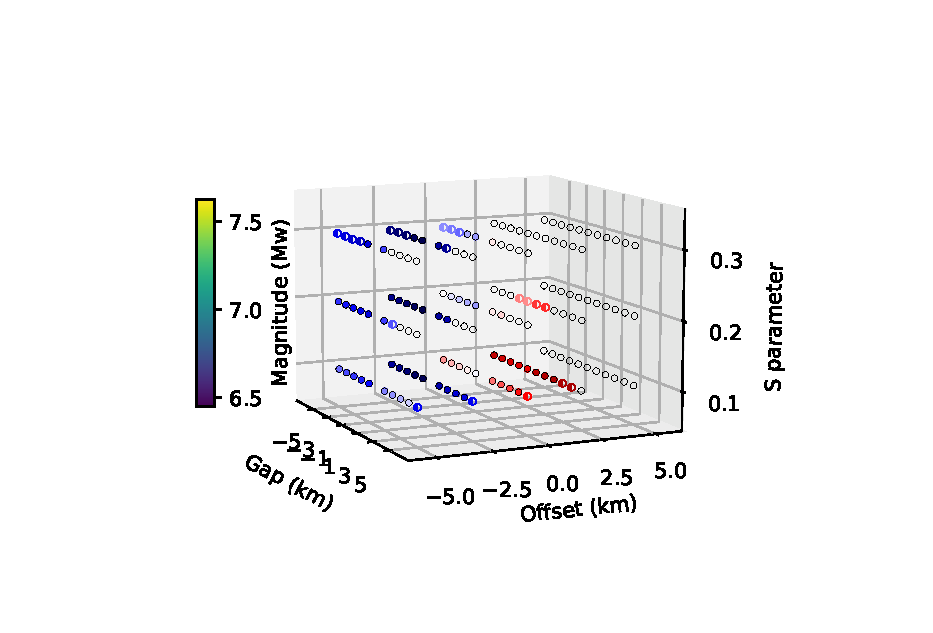
\includegraphics[width=1\linewidth]{images/tests_shmax340}
\end{minipage} 
\hskip 0.3cm \begin{minipage}{0.55\linewidth}

\vskip 0.2cm
156 Simulations were performed using this configuration, where $S$ depends only \\
on the stress level and not on $\mu_s$ or $\mu_d$. In some cases, the rupture did not fully \\ 
break both faults, mainly due to the pre-stress level of the faults.\\
\vskip -0.2cm
\textbf{\small Hanging/foot wall asymmetry:} \\
\vskip -0.3cm
A small asymmetry regarding the triggering potential of the secondary fault \\ 
related to its location with respect to the main fault (hanging or foot wall)\\ 
is observed. When the secondary fault is on the hanging wall, the dynamica-\\
lly triggered rupture is more likely to be self-sustainable. \\
\vskip -0.2cm
\textbf{\small Stress shadow:} \\
\vskip -0.3cm
The final energy released (estimated magnitude) increases/decreases according \\
to the distance between faults (i.e. offset and gap). Although the overlap in-\\
creases the triggering effect, the stress shadow, due to the fault proximity, in-\\
hibits a large stress drop on the secondary fault.



\end{minipage}

}



\headerbox{{\bf 4.} Jump ? How ? When ? Why ?}{name=snaps,column=1,row=1,span=2,below=summary}{

\begin{minipage}{0.48\linewidth}
 \centering {\bf Fault not fixed ($\mu_s=0.6$)}
 \includegraphics[width=0.94\linewidth]{images/horizontal_delta_00018_nofis.png}
\end{minipage} \vrule width 0.05cm
\begin{minipage}{0.48\linewidth}
 \centering {\bf Fault fixed ($\mu_s=50.0$)}
\includegraphics[width=0.94\linewidth]{images/horizontal_delta_00018_nofis.png} 
\end{minipage}\\
\begin{minipage}{0.48\linewidth}
 \centering 
 \includegraphics[width=0.94\linewidth]{images/horizontal_delta_00018_nofis.png}
\end{minipage} \vrule width 0.05cm
\begin{minipage}{0.48\linewidth}
\end{minipage}

}


%\headerbox{{\bf 5.} Results}{name=results,column=1,row=2,span=1,above=bottom}{

%}


\headerbox{\,}{name=snaps,column=2,row=1,span=1,above=bottom}{

\nocite{Improta_2019_AVN}
\nocite{Bernard_1989_IRPINIA}
\nocite{Valoroso_2013_AQUILA}

\vskip -0.7cm
    {\tiny
    \begin{spacing}{1.0}
     \bibliography{biblio/bibtemp} 
    \end{spacing}
    }							
    \bibliographystyle{apalike}    
    

}



\end{poster}
\end{document}





\vskip -0.15cm
 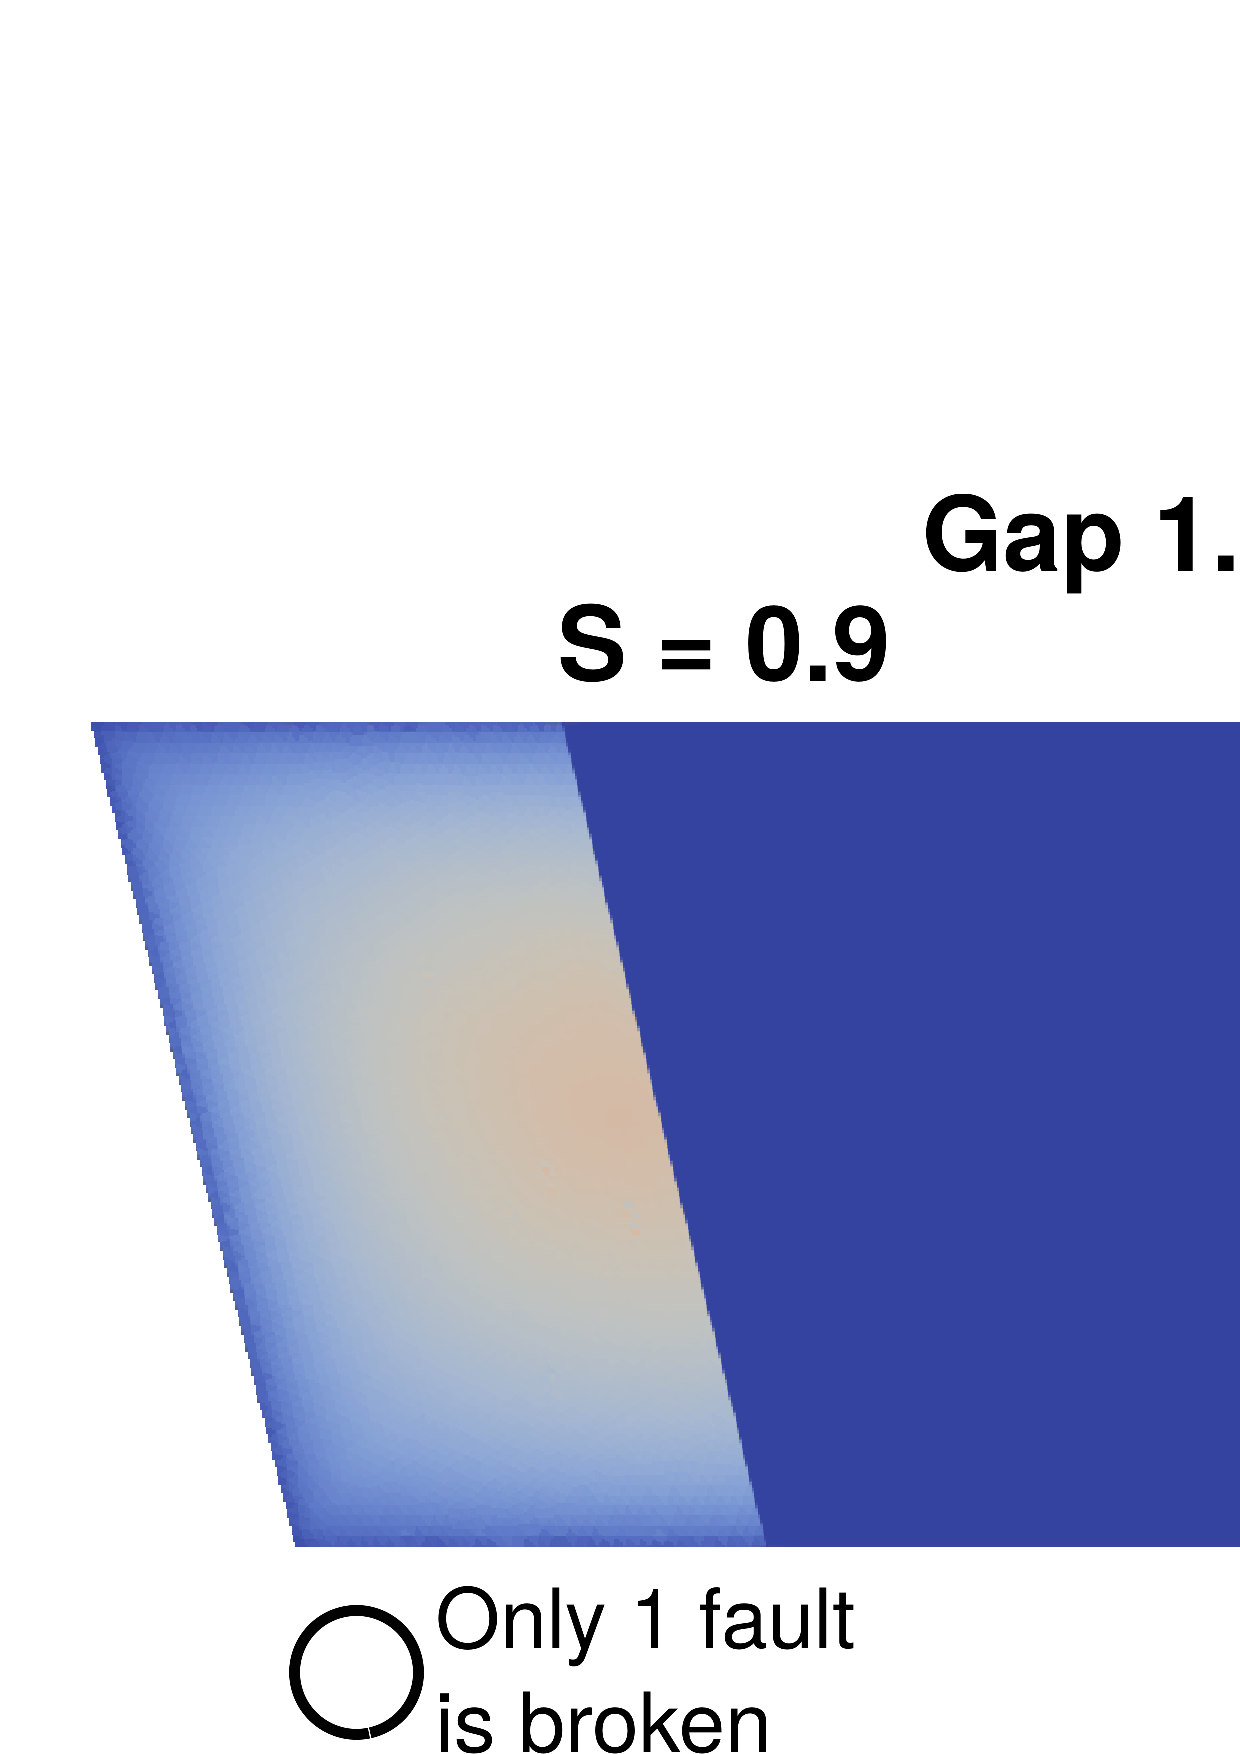
\includegraphics[width=1\linewidth]{images/ruptures.pdf}
 \vskip 0.1cm
 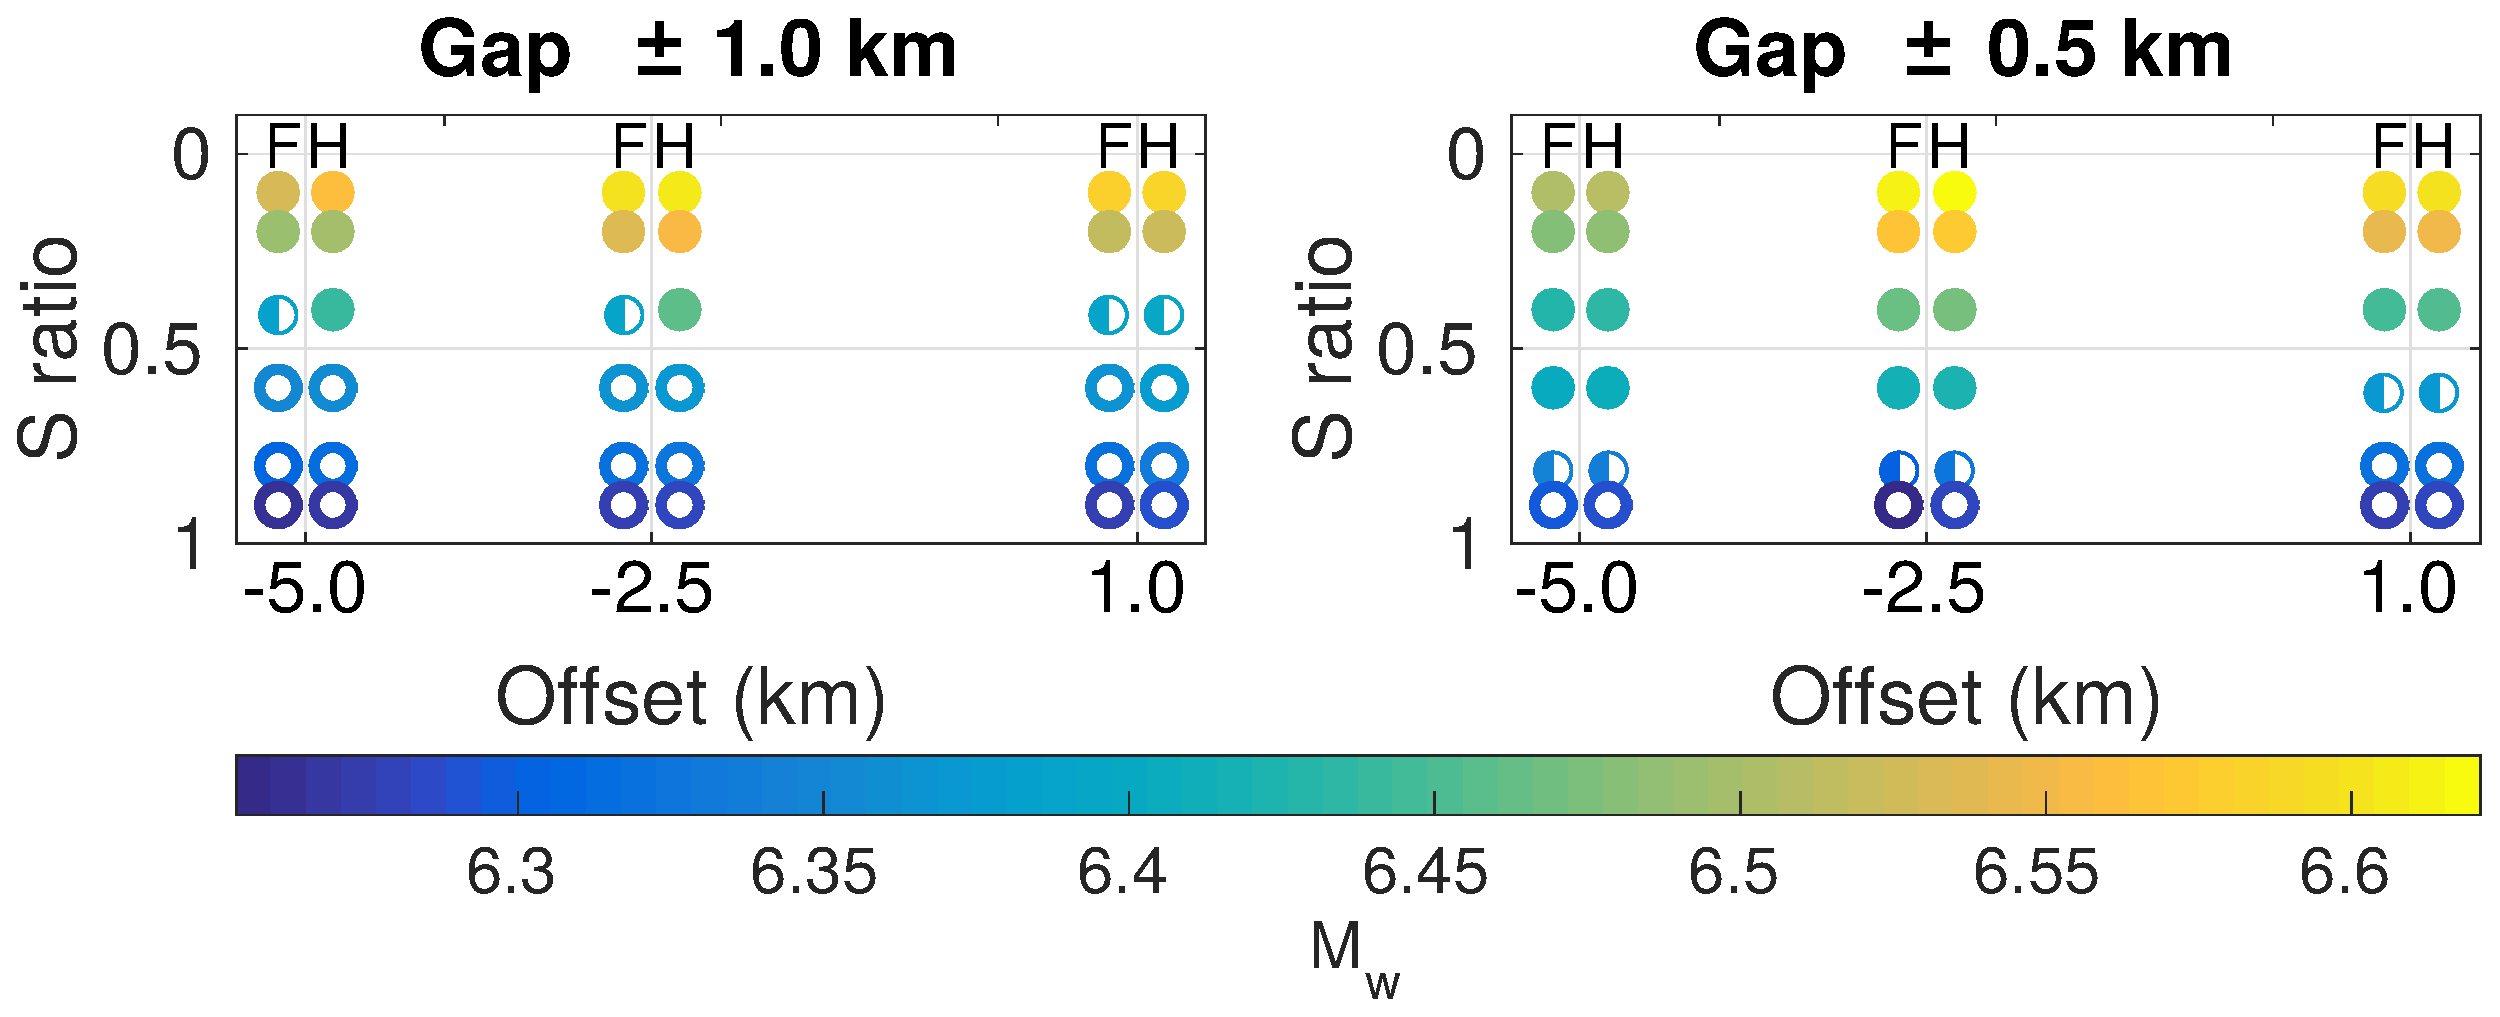
\includegraphics[width=1\linewidth]{images/results_table} \\
\vskip 0cm
\textbf{\small Hanging/foot wall asymmetry:} \\
\vskip -0.3cm
{\small A small asymmetry regarding the triggering potential of the secondary fault related to its location with respect to the main fault (hanging or foot wall) is observed. When the secondary fault is on the hanging wall, the dynamically triggered rupture is more likely to be self-sustainable.} \\
\vskip 0cm
\textbf{\small Stress shadow:} \\
\vskip -0.3cm
The final energy released (estimated magnitude) increases/decreases according to the distance between faults (i.e. offset and gap). Although the overlap increases the triggering effect, the stress shadow, due to the fault proximity, inhibits a large stress drop on the secondary fault.
\begin{center}
 \textbf{Could this triggering be controlled by \\ an static or dynamic Coulomb stress change?}
\end{center}
